\chapter{The SMBO Paradigm}\label{ch:smbo}

To formalize the notion of blackbox optimization, consider an expensive blackbox function $f$. I will also refer to $f$ as the \emph{objective function}, a term from the optimization and statistics communities. Say that $f$ has been evaluated on the inputs, or \emph{sample points}, $x^1,\ x^2, ... ,\ x^n$. These evaluations produce the observed outputs $y^i=f(x^i)$. If $\X=\{x^1, ... ,\ x^n\}$ and $\Y=\{y^1, ...,\ y^n\}$, I'll refer to the pair $(\X,\Y)$ as the \emph{sample data}. Because we are concerned with global optimization---without loss of generality, say minimization\footnote{In the optimization community, it is common to speak only of minimization, and the two words are used somewhat interchangeably. For example, the most popular Python library for optimization, \texttt{scipy.optimize}\cite{scipy_optimize}, contains only minimization routines. Of course, the task of maximizing a function $f$ is the same as minimizing its negative $-f$. }---the goal is to find an $x$ such that $f(x)<f(x')$ for all $x' \ne x$, while evaluating $f$ as few times as possible. This chapter describes formally how the SMBO process addresses this challenge. I will define notation as it is introduced, though for reference I have included a reference table of variable names and definitions in Figure \ref{fig:notation} below.
% Where does this important aside go?: It should be clear that, unless you have evaluated the black box function $f$ at every possible $x$, it is impossible to say with absolute certainty whether a given point is the global minimum. Thus, the goal of a statistical global optimization routine is to produce a candidate optimum $x$, with some measure of confidence that $x$ is in fact the global optimum.

\begin{minipage}{\textwidth}
\begin{framed}
\begin{description}
  \item[$f$]: the objective function
  \item[$k$]: the dimensionality of $f$'s domain
  \item[$x$]: a generic point in $f$'s domain
  \item[$n$]: the number of sample points (points at which $f$ has been evaluated and $f(x)$ is known)
  \item[$x^i$]: the $i$th sample point (a $k$-vector)
  \item[$\X$]: the vector of sample points whose $i$th element is $x^i$ ($n$ $k$-vectors, an $n\times k$ matrix)
  \item[$y^i$]$:= f(x^i)$; the known objective output at the $i$th sample point (a real number)
  \item[$\Y$]: the vector of known outputs (an $n$-vector).
  \item[$\hat{f}(x)$]: the $k$-to-$1$-dimensional predictor function
  \item[$\err(x)$]: the predicted (mean-squared) error of $\hat{f}(x)$; also a $k$-to-$1$-dimensional function
  \item[$y(x)$]$:=$Normal$(\hat{f}(x),\err(x))$; a random variable with mean $\hat{f}(x)$ and standard deviation $\err(x)$, representing the prediction at $x$.
\end{description}


\end{framed}
\captionof{figure}{Notation used throughout this thesis}
\label{fig:notation}
\end{minipage}

\section{The SMBO Loop}

`SMBO' describes an entire class of algorithms, rather than one in particular \cite{hutter_sequential_2011, hamadi_autonomous_2012, jones_efficient_1998, rasmussen_gaussian_2006}. %note: get more specific with those cites. should be a handful of specific papers presenting particular SMBO things
These algorithms differ along several dimensions: in their assumptions regarding determinism, the types of objective functions they can optimize, their modelling strategies, and the details of their interactive relationship to the objective functions being optimized, to name several. % clarification: such as some algorithms selecting one sample point, others more.
Across these differences, the defining feature of sequential model-based optimization can be described as a three-part loop, shown below.

\begin{minipage}{\textwidth}
\begin{framed}

\begin{enumerate} 
\item The objective function $f$ is evaluated at a set of input values $\mb{x}$, producing observed outputs $\mb{y}$.
\item A prediction model of the objective function, the ``predictor function'' $\hat{f}$ is fit to the sample points $(\mb{x},\mb{y})$, as well as a model of the expected error of $\hat{f}$, $\err$.
\item From considering the prediction surface and its error, $(\hat{f},\err)$, new input points $\mb{x_{new}}$ are chosen to be evaluated by $f$. These points are chosen to most improve the ability of the model $\hat{f}$ to find the global optimum.\end{enumerate}
\end{framed}

\captionof{figure}{The three-stage SMBO loop}
\label{fig:smbo_loop}
\end{minipage}
I'll call this three-part process the \emph{SMBO loop} or \emph{cycle}; it will be referenced throughout this thesis. 

Note that at every iteration of the SMBO loop, (presuming we are minimizing $f$) there is a current `incumbent minimum', the best sample point evaluated so far. I will denote this point $x_{min}$, and its associated objective value $y_{min}$:

\begin{align} \label{x_min}
x_{min} &= x_j \in \mb{x}\ |\ y_j \leq y_i\ \ \forall\ y_i \in \mb{y}\\
y_{min} &= f(x_{min}).
\end{align}

The SMBO loop returns $(x_{min},y_{min})$ once $y_{min}$ is satisfactory, which could be defined one of two obvious ways. If we are looking only for `good enough' performance in the blackbox function, then the halting criteria is once the incumbent $y_{min}$ drops below a set threshold, e.g., ``run the SMBO loop until you can find a blackbox value lower than $2$.'' Note that in general with a blackbox function, you can never be certain to have found the global optimum, unless you have sampled every point in the function's domain. Thus, the alternative to using a $y_{min}$ threshold as a halting criteria must be probabilistic---as will be described further in Section \ref{sec:max_imp}, from the prediction surface and its error function $(\hat{f},\err)$, we can rigorously predict the probability that the current $y_{min}$ is in fact the function's global minimum. Thus, it is straightforward to say, ``run the SMBO loop until you are 95\% confident that you have found the global minimum.''

\section{Visualizing the SMBO Loop}

The cyclical nature of sequential model-based optimization suggests a popular illustration of the method, which highlights how the three steps reinforce each other to generate successively more predictive models---see Figure \ref{fig:smbo_cycle}, below. It is somewhat notable that illustrations quite similar to Fig. \ref{fig:smbo_cycle} appear throughout the literature related to SMBO \cite{hutter_sequential_2011,protolife_pdt_2013}. This image is perhaps the most popular conceptualization of the SMBO method.

\begin{figure}[h]
	\centering
	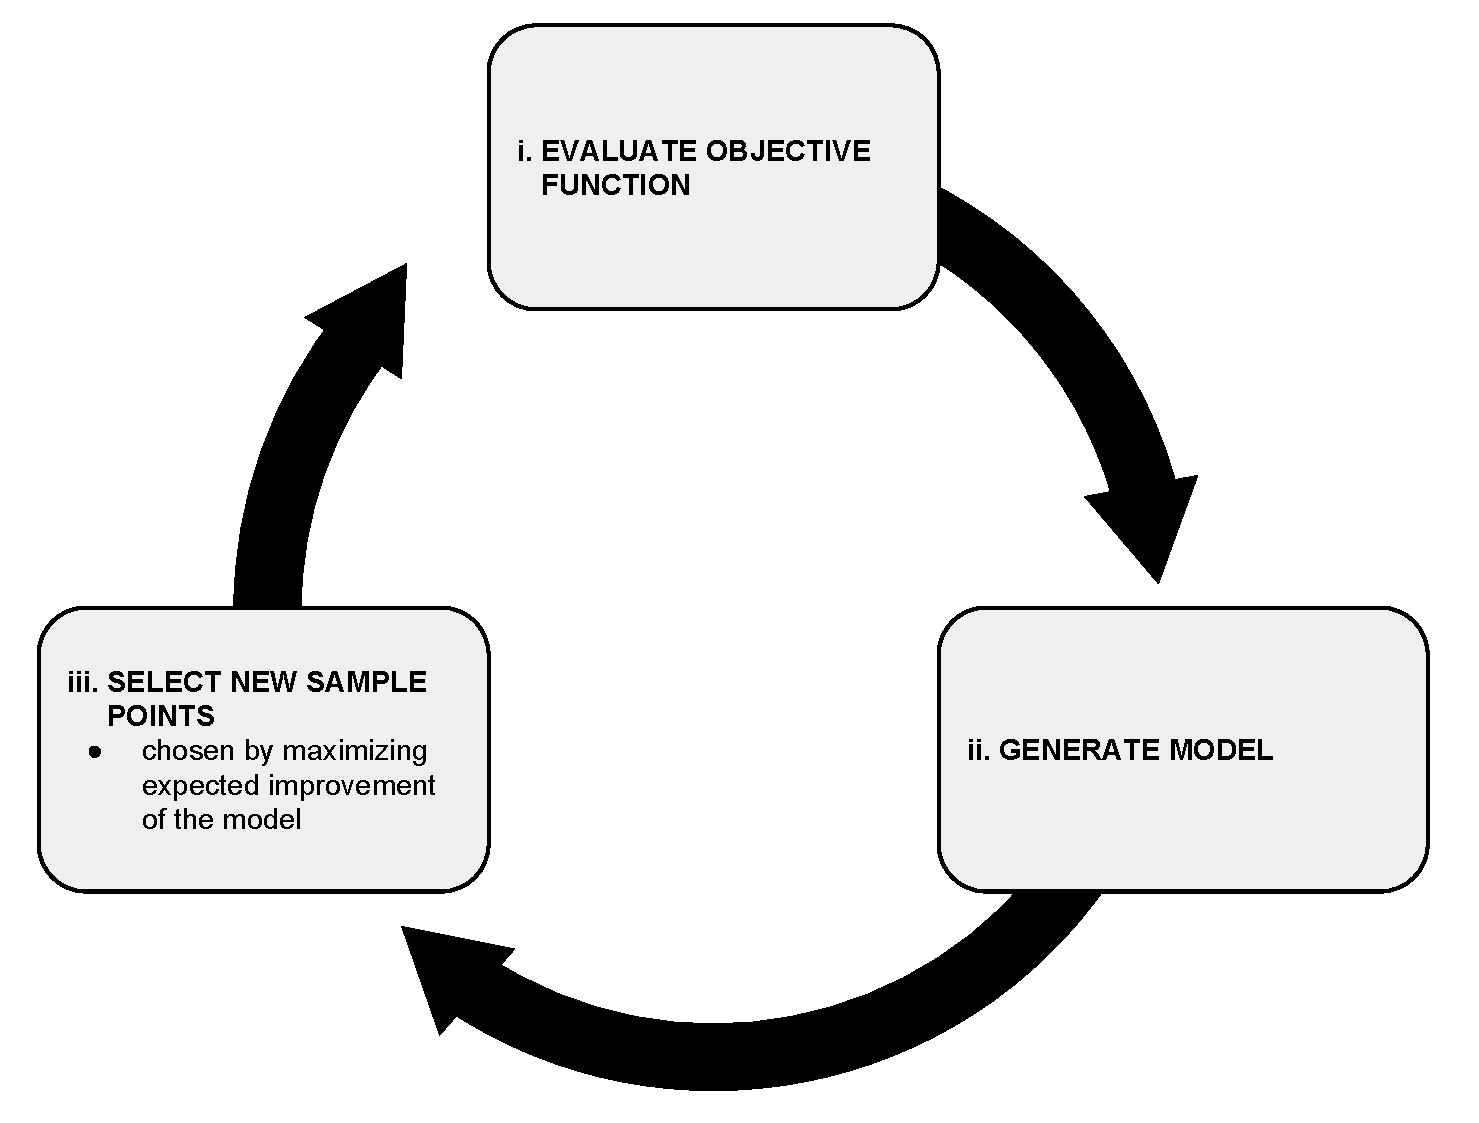
\includegraphics[width=0.75\textwidth]{images/smbo_loop}
	\caption{A popular visualization of the SMBO process. The methodology of node iii is largely fixed across different SMBO algorithms, while the details of Node ii are generally the distinguishing factors between different SMBO algorithms.}
	\label{fig:smbo_cycle}

\end{figure}


%In the vocabulary of above, each stage in the SMBO loop can be defined as a mathematical function:
%\begin{description}
%	\item[\textbf{I}]: The objective function maps $k$-vectors from input-space to outputs.
%	\item[\textbf{II}]: The model module maps the sample points to a model function.
%	\item[\textbf{III}]: The sampling strategy is a function that takes as input a model function, and outputs the next $k$-vector(s) which should be evaluated by the objective.
%\end{description}

%Seeing each component as simply a function mapping a certain kind of input to a certain kind of output, combined with the circular relationship illustrated in Fig \ref{fig:smbo_cycle}, is what motivates me to describe the SMBO process as bootstrapping. From the perspective of node \textbf{I} in the cycle, the output of the objective function determines the next input of the objective function, which determines the next input, and do on. From the perspective of node \textbf{II}, each model induces the model that follows it.

\section{SMBO$_{\text{III}}$: Maximum Improvement}\label{sec:max_imp}

The third step in the SMBO loop is perhaps the most characteristic---different SMBO algorithms use different model functions to accomplish the task in node \textbf{II}, and of course each implementation might attempt to optimize a unique objective function in step \textbf{I}. The third step, however, has a standard solution that is relatively ubiquitous: maximizing a function of input space called \emph{expected improvement}. 

There is a classical problem in optimization, of balancing the competing desires for exploration and exploitation \cite{John Holland}. Here, exploration refers to the impulse to sample in unknown regions of the objective function's domain, to learn more about its global behavior. Exploitation means the impulse to take advantage of what we already know, and sample where we predict we will find the global optimum. Expected improvement is one of those results from statistics that does a strikingly good job of quantifying a concept that seems at first to be too subtle to be easily quantified---it provides a satisfying solution to the exploration/exploitation conundrum.

Remember that during the SMBO process (as in many other optimization strategies), there is at all times a current ``incumbent optimum,'' $(x_{min},y_{min})$, which is the most optimal sample point evaluated so far. Simply put, the expected improvement of $x'$ measures amount by which we predict that $f(x')$ would be more optimal than $y_{min}$. More rigorously, improvement $I$ is defined as,

\begin{equation} \label{eq:improvement}
I(x) = min(y_{min}-y(x),0),
\end{equation}
where I have defined $y(x)=\text{Normal}(\hat{f}(x),\err(x))$; thus $I$ is a random variable. It should be clear to the reader that $I$ does capture the intuitive notion of improvement---it is the amount by which $y(x)$ is better than the incumbent optimum.

From this definition of improvement, all that is left is to apply the basic statistical notion of the expected value of a random variable to Eq. \ref{eq:improvement} to find the expected improvement function $\mb{E}[I(x)]$. Doing this, along with what \cite{jones_efficient_1998} calls `some tedious integration by parts,' produces the formula,

\begin{equation} \label{eq:exp_improvement}
\mb{E}[min(y_{min}-y(x),0)]=(y_{min}-\hat{f}(x))\times\Psi\left(\frac{y_{min}-\hat{f}(x)}{\err(x)}\right) + \err(x)\times\psi\left(\frac{y_{min}-\hat{f}(x)}{\err(x)}\right),
\end{equation}
where $\Psi$ and $\psi$ denote the standard normal distribution and density functions, familiar from statistics.

A significant feature of expected improvement is that it is monotonic in both $\err$ and $\hat{f}$. Ignoring $\hat{f}(x)$, if a prediction is uncertain (measured by $\err(x)$), then the expected improvement will be large. On the other hand, if we ignore predicted error, it is obvious that the points in input space where $\hat(x)$ is lower will have a higher expected improvement (assuming the goal is minimization). 

By choosing sample points to maximize the expected improve function, exploration and exploitation go hand in hand. This is easier illustrated than described, so I have included in Figure \ref{fig:explore_exploit} the plots from a toy SMBO instance where the exploration/exploitation distinction is was especially prominent.


\begin{figure}
\centering
\begin{tabular}{lr}
\subcaptionbox{The initial model, fit only on a 4-point latin hypercube sample.}
{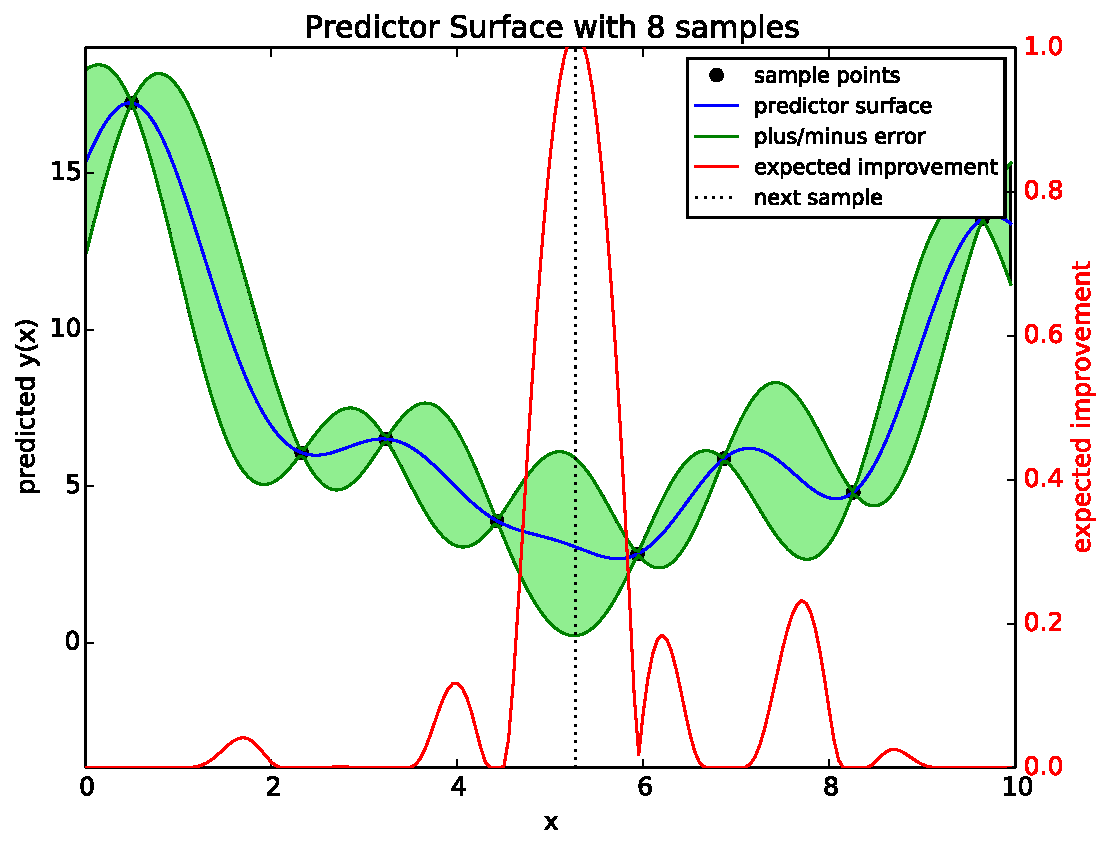
\includegraphics[width=0.4\textwidth]{images/ego_ex/0}} &

\subcaptionbox{Note that the new sample point is very near the global minimum.}
{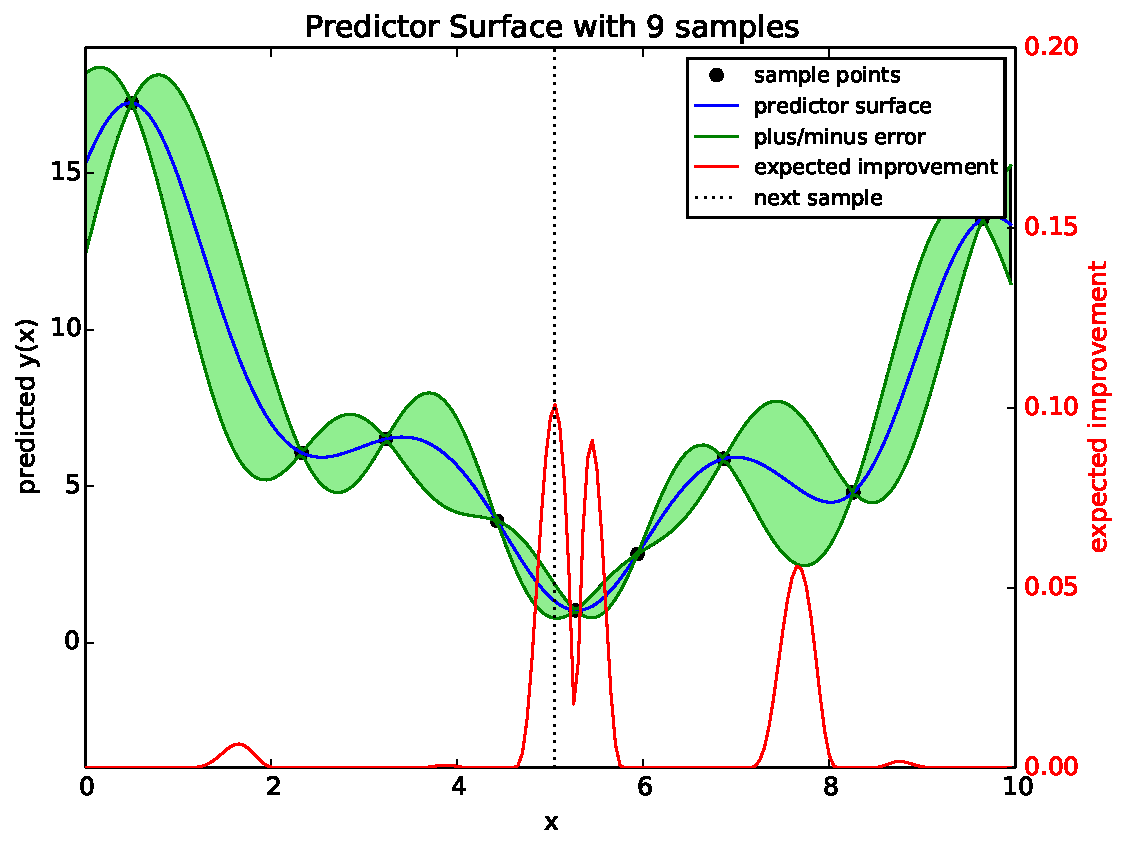
\includegraphics[width=0.4\textwidth]{images/ego_ex/1}}\\

\subcaptionbox{Despite the good result found in (b), the predictor is very uncertain in the unexplored region, so the expected improvement is largest there---it is now exploring rather than exploiting.}
{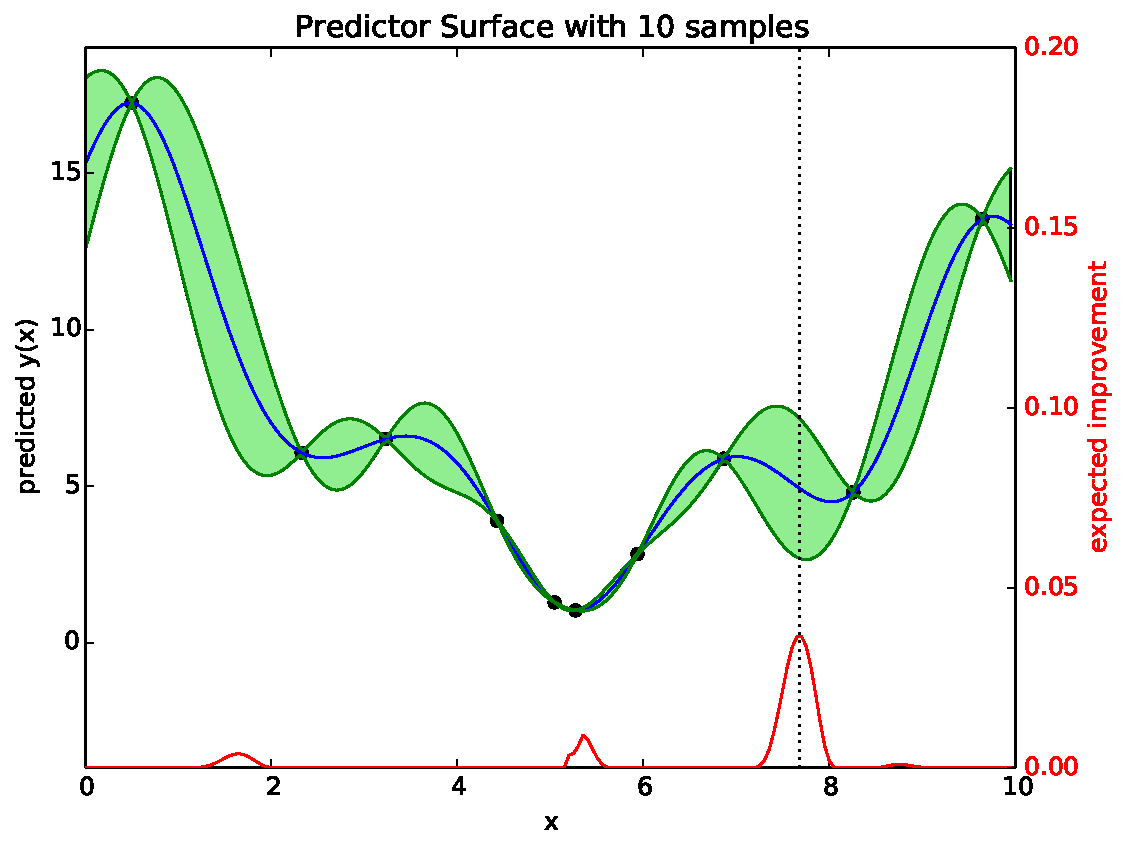
\includegraphics[width=0.4\textwidth]{images/ego_ex/2}} &

\subcaptionbox{More exploration of the uncertain region}
{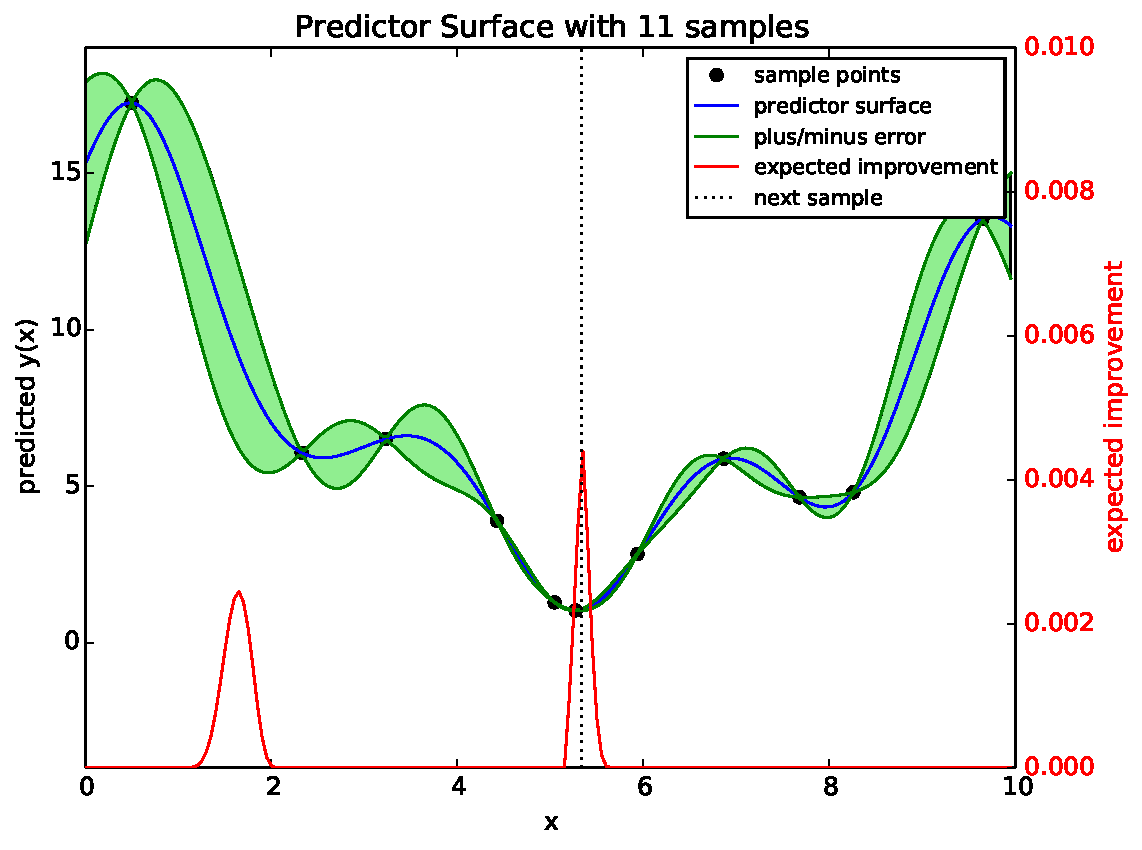
\includegraphics[width=0.4\textwidth]{images/ego_ex/3}}\\

\subcaptionbox{Now that the domain is more fully mapped, the algorithm is more confident that the solution in (b) is close to the global minimum}
{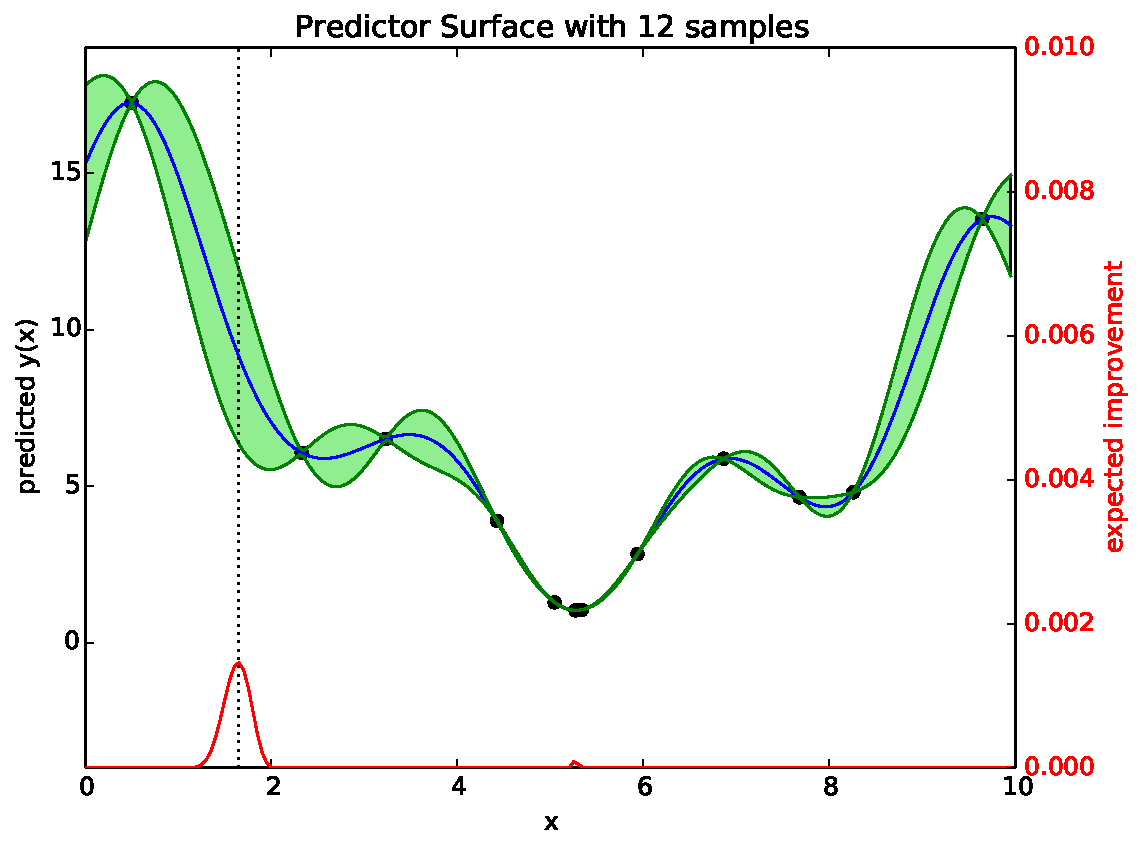
\includegraphics[width=0.4\textwidth]{images/ego_ex/4}} &

\subcaptionbox{Note that despite uncertain regions of the prediction surface, nowhere is it very likely that a new sample would find a better $y_{min}$.}
{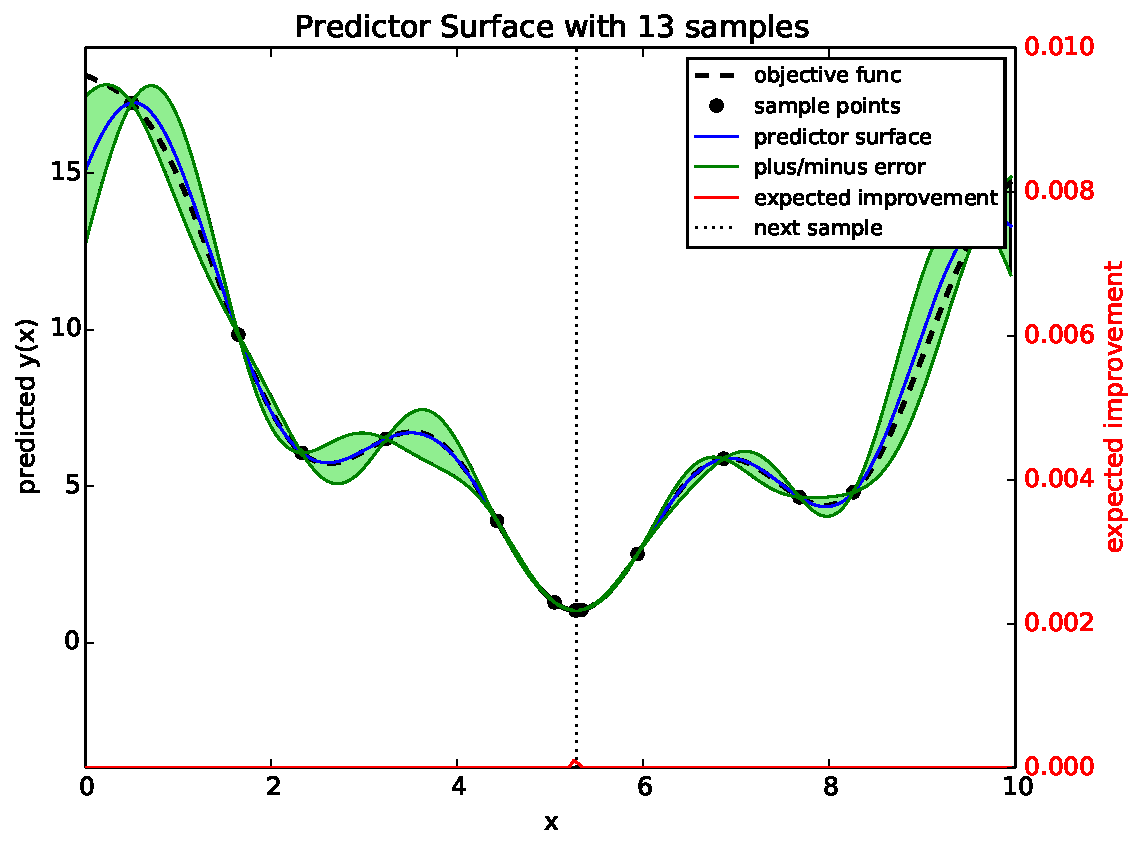
\includegraphics[width=0.4\textwidth]{images/ego_ex/5}}\\
\end{tabular}
\caption{An entire run of sequential model-based optimization of a toy function using the EGO algorithm, highlighting the exploration/exploitation tradeoff achieved by when maximum expected improvement is used to select $x_{new}$.}
\label{fig:explore_exploit}
\end{figure}


\section{SMBO$_0$: The Initial Sample}

Obviously, it is impossible to construct a model of a blackbox function's response surface if you have not ever queried the function at all, so the SMBO loop cannot start itself without a strategy for picking initial sample points. A popular strategy (find sources on wikipedia) for selecting these points, and the only strategy I will consider in this thesis, is called a latin hypercube sample. I will briefly describe it here, though the specific sampling method is not of great conceptual importance.

To construct an $n$-point latin hypercube in $k$ dimensions, first divide each dimension's domain into $n$ rows. This induces a grid, subdividing the original $k$-rectangular domain into $n^k$ sub-rectangles. A latin hypercube sample takes points from this domain under the constraint that no row in any one dimension contains two sample points.

That being said, the latin hypercube is one of those things that is more easily explained with pictures than words. [Put pictures here: is it cool to just life (and cite) the wikimedia commons pics from wikipedia?].

If you are a fan of sudoku, you have spent a lot of time thinking about latin hypercubes: the distribution of any one numeral across the game board matches a nine-sample two-dimensional latin hypercube. [Little picture demonstrating this, perhaps in a row with the wikipedia latin squares]







